\documentclass[11pt]{article}

\usepackage[utf8]{inputenc}
\usepackage[T1]{fontenc}
\usepackage{lmodern}
\usepackage[a4paper,margin=2.5cm]{geometry}
\usepackage{amsmath,amssymb,mathtools,amsthm}
\usepackage{booktabs}
\usepackage{graphicx}
\usepackage{microtype}
\usepackage{enumitem}
\usepackage{url}
\usepackage[hidelinks]{hyperref}

\newtheorem{theorem}{Theorem}
\newtheorem{lemma}{Lemma}
\newtheorem{proposition}{Proposition}
\newtheorem{corollary}{Corollary}

\title{Anytime-Valid Predictive-Rank Detection with a Statically Contaminated Reference Set}
\author{Juan Felipe Orozco Cort\'es}
\date{}

\begin{document}

\maketitle

\begin{abstract}
Sequential distribution-shift detection often relies on a fixed reference sample that represents the nominal distribution. Predictive-rank martingales provide exact anytime-valid monitoring when that reference is clean, but in radar, monitoring, and calibration systems the reference bank itself may contain persistent interferers or outliers. We study a finite fixed reference containing an unknown set of static, exogenous replacements whose identities remain unchanged throughout online monitoring. For every candidate set of contaminated sorted positions, we reconstruct a candidate clean-reference rank sequence and apply a valid predictive-rank betting construction. The true candidate recovers the clean rank process exactly; consequently, the pointwise lower envelope of candidate wealths is pathwise dominated by a valid clean predictive-rank martingale, yielding finite-sample anytime threshold-crossing control without estimating the unknown null distribution. A corollary extends validity from a known contamination count to a known upper bound. The static contamination pattern also induces a contiguous-partition structure on observed-rank bins, yielding an exact \(O(Km^2)\) dynamic program for a fixed categorical bettor. In a post-freeze Monte Carlo validation with 5,000 replications per condition, \(K=32\), \(m=2\), \(T=200\), and a \(\mathrm{Beta}(4,1)\) shift, the proposed method crosses with probability \(0.9144\) (95\% CI \(0.9063\)--\(0.9218\)), versus \(0.1152\) for a fixed confidence-band comparator and \(0.9810\) for the oracle. A preregistered contamination-geometry stress test retained static crossing probabilities between \(0.8894\) and \(0.9468\) across upper in-support, mixed-tail, and independently random static contamination, while the fixed comparator rose to \(0.2162\)--\(0.3948\). Separate semi-synthetic RTL-SDR experiments with real receiver/background IQ and controlled post-ADC injection reproduced the qualitative sensitivity advantage, including a non-saturated transition at \(-18\) and \(-15\) dB. These experiments are engineering sensitivity checks rather than hardware type-I validation. Overall, the results support a finite-reference advantage from exploiting persistent contamination identities rather than representing contamination only as generic CDF uncertainty.
\end{abstract}

\noindent\textbf{Keywords:} anytime-valid inference; predictive ranks; martingales; e-values; contaminated reference data; CFAR; distribution-shift detection; robust statistics.

\section{Introduction}
% Source prose: docs/manuscript/abstract_introduction_v0_1.md
% Next pass: convert frozen Introduction and replace citation placeholders with BibTeX keys.

\section{Problem Formulation and Predictive-Rank Background}

\subsection{Fixed reference with static contamination}

Let the observed reference bank contain \(K\) scalar observations. Exactly \(m\) are contaminated and
\[
  n=K-m
\]
are clean. Let \(G\subseteq\{1,\ldots,K\}\), \(|G|=n\), denote the unknown set of clean physical reference-cell identities and \(B=G^c\), \(|B|=m\), the contaminated physical cells. For every \(i\in G\),
\[
  Y_i\overset{\mathrm{iid}}{\sim}F,
\]
where \(F\) is an unknown continuous distribution. The online null stream satisfies
\[
  X_1,X_2,\ldots\overset{\mathrm{iid}}{\sim}F
\]
independently of the clean reference observations.

The contaminated values \(\{Y_i:i\in B\}\) may be arbitrary, but the contamination is \emph{static and exogenous}: the contaminated physical cells are fixed before monitoring begins, and the surviving clean sample is not selected adaptively after inspecting the realized clean values. The theory therefore does not cover the stronger model in which an adversary first observes \(K\) clean draws and then chooses which realized values to replace. Such selection can bias the surviving clean subset.

Continuity of \(F\) implies that clean-reference and future-null ties occur with probability zero. Randomized tie-breaking independent of the data can be added if required by an implementation.

\subsection{Sorted reference representation}

Let
\[
  Z_{(1)}\le\cdots\le Z_{(K)}
\]
be the sorted observed reference values. The contaminated physical cells occupy an unknown realized set of sorted positions
\[
  C^\star\subseteq\{1,\ldots,K\},
  \qquad |C^\star|=m.
\]
The set \(C^\star\) can be random because sorting depends on the realized clean and contaminated values. Deleting those realized positions nevertheless recovers the original iid clean sample.

For an online observation \(X_t\), define the observable full-reference rank
\[
  Q_t
  =
  \#\{i:Z_{(i)}\le X_t\}
  \in\{0,\ldots,K\}.
\]

\subsection{Candidate contamination sets}

Let
\[
  \mathcal C_m
  =
  \{C\subseteq\{1,\ldots,K\}:|C|=m\}.
\]
For \(C\in\mathcal C_m\), define the reconstructed candidate rank
\begin{equation}
  R_t^{(C)}
  =
  Q_t-\#\{c\in C:c\le Q_t\}
  \in\{0,\ldots,n\}.
  \label{eq:candidate-rank}
\end{equation}

\begin{lemma}[True-candidate rank reconstruction]
Under the static/exogenous contamination model,
\begin{equation}
  R_t^{(C^\star)}
  =
  \#\{i\in G:Y_i\le X_t\}
  \qquad\text{for every }t.
  \label{eq:true-reconstruction}
\end{equation}
\end{lemma}

\begin{proof}
The full rank \(Q_t\) counts every observed reference not exceeding \(X_t\), including clean and contaminated values. Among those counted observations, exactly \(\#\{c\in C^\star:c\le Q_t\}\) occupy contaminated sorted positions. Subtracting them leaves precisely the number of clean references not exceeding \(X_t\).
\end{proof}

\subsection{Clean fixed-reference predictive ranks}

We recall the clean predictive-rank result of Kuang and Xia \cite{KuangXia2026}. Let \(Y_1,\ldots,Y_n,X_1,X_2,\ldots\) be iid from continuous \(F\), and define
\[
  R_t=\#\{i:Y_i\le X_t\},
  \qquad
  N_{j,t-1}=\sum_{s<t}\mathbf 1\{R_s=j\}.
\]
With \(\mathcal G_t=\sigma(R_1,\ldots,R_t)\), the exact predictive null law is
\begin{equation}
  \Pr(R_t=j\mid\mathcal G_{t-1})
  =
  p_{t,j}
  =
  \frac{N_{j,t-1}+1}{n+t},
  \qquad j=0,\ldots,n.
  \label{eq:predictive-null}
\end{equation}
This result is distribution-free. A standard derivation maps the clean reference through the probability integral transform; the \(n+1\) uniform spacings have a \(\mathrm{Dirichlet}(1,\ldots,1)\) law, and Dirichlet--multinomial prediction yields \eqref{eq:predictive-null}.

The guarantee is marginal over the random fixed reference sample. Conditional on the realized numerical reference values, the rank probabilities are the realized spacing probabilities and are not generally equal to \eqref{eq:predictive-null}.

\subsection{Clean predictive-rank martingales and predictable betting rules}

At time \(t\), let \(q_t=(q_{t,0},\ldots,q_{t,n})\) be a \(\mathcal G_{t-1}\)-measurable probability vector. Equivalently, we may regard the betting strategy as a deterministic measurable map
\[
  \mathsf q_t:
  \{0,\ldots,n\}^{t-1}
  \longrightarrow
  \Delta_n,
\]
where \(\Delta_n\) is the probability simplex on \(\{0,\ldots,n\}\), and set
\[
  q_t=\mathsf q_t(R_1,\ldots,R_{t-1}).
\]
This functional view will be useful under contamination: the same pre-specified map is applied to every candidate reconstructed rank history, and for the true candidate it is automatically predictable with respect to the canonical clean-rank filtration. Define
\begin{equation}
  e_t=\frac{q_{t,R_t}}{p_{t,R_t}},
  \qquad
  E_0=1,
  \qquad
  E_t=\prod_{s=1}^t e_s.
  \label{eq:clean-prm}
\end{equation}
Kuang and Xia \cite{KuangXia2026} show that \((E_t)\) is a nonnegative martingale because
\[
  \mathbb E[e_t\mid\mathcal G_{t-1}]
  =
  \sum_{j=0}^n p_{t,j}\frac{q_{t,j}}{p_{t,j}}
  =1.
\]
Consequently, Ville's inequality gives
\begin{equation}
  \Pr_{H_0}\!\left(
    \sup_{t\ge0}E_t\ge\frac1\alpha
  \right)\le\alpha.
  \label{eq:ville-clean}
\end{equation}

The frozen empirical method uses a fixed convex portfolio of PRM wealth processes together with a \(5\%\) constant-one hedge. Convex PRM portfolios are prior art/standard martingale closure and are not claimed as novel here.


\subsection{Canonical clean-rank process}

Under the contaminated-reference model, define the latent canonical clean rank
\begin{equation}
  R_t^\star
  =
  \#\{i\in G:Y_i\le X_t\},
  \qquad
  \mathcal G_t^\star
  =
  \sigma(R_1^\star,\ldots,R_t^\star).
  \label{eq:canonical-clean-rank}
\end{equation}
By Lemma~1,
\[
  R_t^{(C^\star)}=R_t^\star
\]
pathwise for every \(t\).

For a candidate \(C\in\mathcal C_m\), we apply the same deterministic betting maps to its reconstructed history:
\[
  q_t^{(C)}
  =
  \mathsf q_t
  \!\left(
    R_1^{(C)},\ldots,R_{t-1}^{(C)}
  \right).
\]
Consequently,
\[
  q_t^{(C^\star)}
  =
  \mathsf q_t(R_1^\star,\ldots,R_{t-1}^\star)
\]
is \(\mathcal G_{t-1}^\star\)-measurable. Thus the true-candidate wealth is a martingale with respect to the canonical clean-rank filtration \((\mathcal G_t^\star)\); no filtration containing the numerical reference vector is required.

\section{Robust Anytime-Valid Detection under Static Reference Contamination}
% Source: docs/manuscript/sections_2_3_v0_1.md

\section{Experimental Design}

\subsection{Goals and data-generating model}

The experiments evaluate finite-reference power rather than establish validity, which follows from Theorem~1. The final frozen comparisons use
\[
  K\in\{24,32\},\qquad m=2,\qquad n=K-2,
\]
with clean reference values \(Y_i\sim\mathrm{Uniform}(0,1)\). The two contaminated references are fixed at value \(2\). Under the null,
\[
  X_t\sim\mathrm{Uniform}(0,1),
\]
and under alternatives
\[
  X_t\sim\mathrm{Beta}(\gamma,1),
  \qquad \gamma\in\{2,4,8\}.
\]
The maximum horizon is \(T=200\), with intermediate reporting at \(T\in\{40,100,200\}\), and the nominal anytime level is \(\alpha=0.05\). All methods use identical simulated paths within each replication.

\subsection{Static-coupling method and oracle}

For each path, every candidate set \(C\subseteq\{1,\ldots,K\}\) with \(|C|=2\) is evaluated. Candidate ranks are given by \eqref{eq:candidate-rank}, the frozen predictive-rank portfolio is applied, and the robust statistic is \(\underline E_t\). A detection occurs when
\[
  \underline E_t\ge20.
\]

The oracle knows \(C^\star\) and applies the same betting portfolio directly to the true clean rank sequence. Its threshold is also 20. It quantifies the cost of unknown contamination identities.

\subsection{Confidence-band baselines}

The comparison baselines discard contamination identities and represent reference uncertainty through simultaneous CDF bounds. Let
\[
  q(x)=\#\{\text{all }K\text{ observed references}\le x\}.
\]
Because exactly \(m\) observations are arbitrary replacements,
\[
  \max\{0,q(x)-m\}
  \le q_{\mathrm{clean}}(x)
  \le \min\{n,q(x)\}.
\]
For DKW radius
\[
  \epsilon_n(\delta)
  =
  \sqrt{\frac{\log(2/\delta)}{2n}},
\]
the exact-count lower bound is
\begin{equation}
  L_\delta(x)
  =
  \max\left\{
    0,
    \frac{\max(0,q(x)-m)}{n}
    -
    \epsilon_n(\delta)
  \right\}.
  \label{eq:exact-count-band}
\end{equation}

A symmetric contaminated-reference radius follows from
\[
  \widetilde F_K
  =
  \frac nK\widehat F_{\mathrm{clean}}
  +
  \frac mK\widehat F_{\mathrm{bad}},
\]
giving
\begin{equation}
  \epsilon_{\mathrm{sym}}(\delta)
  =
  \frac nK\epsilon_n(\delta)
  +
  \frac mK.
  \label{eq:sym-band}
\end{equation}
This radius is inserted into a one-sided CCTM-style betting geometry. These contaminated-reference constructions are ours for comparison; they are not algorithms claimed by Shaer et al.~\cite{ShaerEtAl2026}.

\subsection{Baseline-strength audit}

The final audit sweeps
\[
  \delta\in
  \{0.005,0.010,0.015,0.020,0.025,0.030,0.035,0.040,0.045\}.
\]
For target marginal level \(\alpha=0.05\), each confidence-band configuration uses
\[
  a(\delta)
  =
  \frac{\alpha-\delta}{1-\delta}
\]
and threshold \(1/a(\delta)\), corresponding to the conservative marginal budget
\[
  a(1-\delta)+\delta\le\alpha.
\]

Three baseline families are evaluated:
\begin{enumerate}[leftmargin=*]
  \item a fixed mixture over \(\eta\in\{0.05,0.10,0.20,0.40,0.60,0.80,0.95\}\) using the signal \(h_t=2(L_\delta(X_t)-1/2)\), with a \(5\%\) constant-one hedge;
  \item one-dimensional online Newton step (ONS) betting with predictable \(\eta_t\in[0,0.99]\) on the same exact-count lower-band signal; and
  \item a one-sided CCTM-style ONS comparator using \eqref{eq:sym-band} with \(D\in\{0.50,0.90,0.99\}\).
\end{enumerate}

For each simulated condition we report the strongest configuration selected \emph{ex post} from this frozen grid. This envelope is not itself one precommitted level-\(\alpha\) test; it is an adversarial descriptive benchmark designed to favor the confidence-band family.

\subsection{Monte Carlo protocol}

The final baseline-strength audit uses 200 Monte Carlo paths per condition with seed \(20260918\). The principal metrics are crossing probability by horizon, median detection delay among detected paths, and median terminal log evidence as a diagnostic.

Delay is conditional on detection and can be selection-biased for methods with very low crossing probability. Terminal log evidence is not directly comparable across methods because tuned confidence-band thresholds depend on \(\delta\), whereas the static and oracle thresholds equal 20.

Before running the final audit, the primary stress point was fixed at
\[
  K=32,\qquad \gamma=4,\qquad T=200,
\]
and a strong empirical pass required
\[
  \widehat P_{\mathrm{static}}
  -
  \widehat P_{\mathrm{strongest\ tuned\ baseline}}
  \ge0.15.
\]
No further bettor or detector tuning was permitted after this criterion was evaluated.

\section{Results}

\subsection{Null sanity check}

The publication-scale null experiment uses 5,000 paths per \(K\). At \(T=200\), observed crossing probabilities for the proposed method are \(0.0112\) (95\% CI \([0.0086,0.0145]\)) for \(K=24\) and \(0.0144\) (95\% CI \([0.0115,0.0181]\)) for \(K=32\). Oracle null crossing probabilities are \(0.0328\) and \(0.0324\), respectively. The strongest frozen-grid confidence-band benchmark has zero crossings in both null settings. These Monte Carlo estimates do not establish validity; they provide an implementation sanity check against the nominal anytime level \(\alpha=0.05\).

\subsection{Crossing probabilities}

Table~\ref{tab:crossing} summarizes the post-freeze publication-scale validation at \(T=200\).

\begin{table}[ht]
\centering
\caption{Crossing probability by \(T=200\) from 5,000 replications per condition. The confidence-band column reports the strongest ex-post configuration in the frozen grid.}
\label{tab:crossing}
\begin{tabular}{llccc}
\toprule
\(K\) & Condition & Static & Best band & Oracle\\
\midrule
24 & null & 0.0112 & 0.0000 & 0.0328\\
24 & \(\mathrm{Beta}(2,1)\) & 0.1824 & 0.0000 & 0.4258\\
24 & \(\mathrm{Beta}(4,1)\) & 0.8758 & 0.0106 & 0.9740\\
24 & \(\mathrm{Beta}(8,1)\) & 0.9980 & 0.3434 & 1.0000\\
32 & null & 0.0144 & 0.0000 & 0.0324\\
32 & \(\mathrm{Beta}(2,1)\) & 0.2036 & 0.0002 & 0.4396\\
32 & \(\mathrm{Beta}(4,1)\) & 0.9144 & 0.1152 & 0.9810\\
32 & \(\mathrm{Beta}(8,1)\) & 0.9998 & 0.8362 & 1.0000\\
\bottomrule
\end{tabular}
\end{table}

At the pre-specified primary point \(K=32,\gamma=4,T=200\),
\[
  \widehat P_{\mathrm{static}}=0.9144,\qquad
  \widehat P_{\mathrm{best\ grid}}=0.1152,\qquad
  \widehat P_{\mathrm{oracle}}=0.9810.
\]
The static 95\% Wilson interval is \([0.9063,0.9218]\). The paired static-minus-baseline gap is \(0.7992\) with 95\% bootstrap interval \([0.7880,0.8104]\), far above the frozen development margin of 0.15. The paired oracle-minus-static gap is \(0.0666\) with 95\% bootstrap interval \([0.0598,0.0736]\).

For the strong \(\gamma=8\) alternative at \(K=32\), static coupling reaches \(0.9998\), the oracle reaches \(1.0000\), and the strongest frozen-grid baseline reaches \(0.8362\). The smaller oracle-static gap is consistent with saturation under a strong signal.

For the weak \(\gamma=2\) alternative, static crossing probability is \(0.1824\) at \(K=24\) and \(0.2036\) at \(K=32\), while the oracle reaches \(0.4258\) and \(0.4396\). Unknown contamination identities therefore impose a substantial finite-reference penalty under weak shifts.

\begin{figure}[ht]
\centering
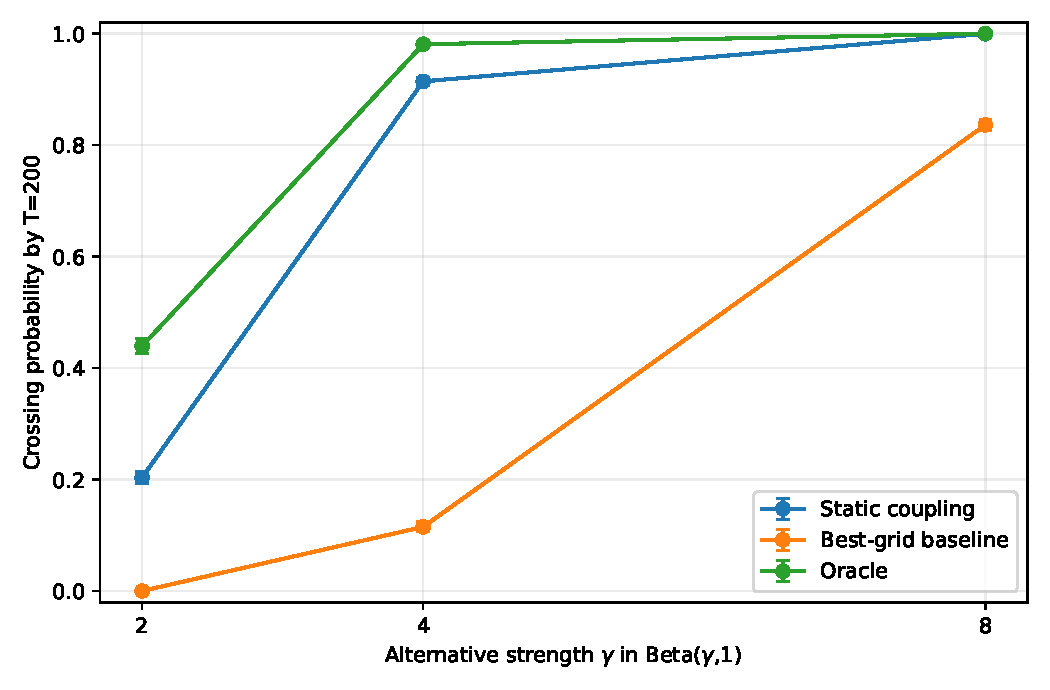
\includegraphics[width=0.82\linewidth]{../results/publication_v1/figures/crossing_T200_K32.pdf}
\caption{Crossing probability by \(T=200\) for \(K=32\), with 95\% Wilson intervals. The confidence-band curve is the strongest ex-post configuration from the frozen baseline grid for each alternative.}
\label{fig:crossing-k32}
\end{figure}

\subsection{Detection delays}

Table~\ref{tab:delays} reports median stopping times among paths that cross by \(T=200\).

\begin{table}[ht]
\centering
\caption{Median detected delay at \(T=200\).}
\label{tab:delays}
\begin{tabular}{llccc}
\toprule
\(K\) & Alternative & Static & Best grid & Oracle\\
\midrule
24 & \(\mathrm{Beta}(2,1)\) & 29 & -- & 17\\
24 & \(\mathrm{Beta}(4,1)\) & 20 & 117 & 9\\
24 & \(\mathrm{Beta}(8,1)\) & 8 & 75 & 5\\
32 & \(\mathrm{Beta}(2,1)\) & 22 & 178 & 16\\
32 & \(\mathrm{Beta}(4,1)\) & 15 & 97 & 8\\
32 & \(\mathrm{Beta}(8,1)\) & 7 & 53 & 4\\
\bottomrule
\end{tabular}
\end{table}

At the primary \(K=32,\gamma=4\) point, the proposed method has median detected stopping time 15 (95\% bootstrap CI \([14.5,16]\)), versus 97 \([92.5,102]\) for the best-grid baseline and 8 \([8,8]\) for the oracle. The \(\gamma=2\) baseline delays are not substantively comparable because the best-grid baseline crosses on zero of 5,000 paths for \(K=24\) and only one path for \(K=32\). Because these medians condition on detection, they are interpreted together with crossing probabilities rather than as standalone speed metrics.

\begin{figure}[ht]
\centering
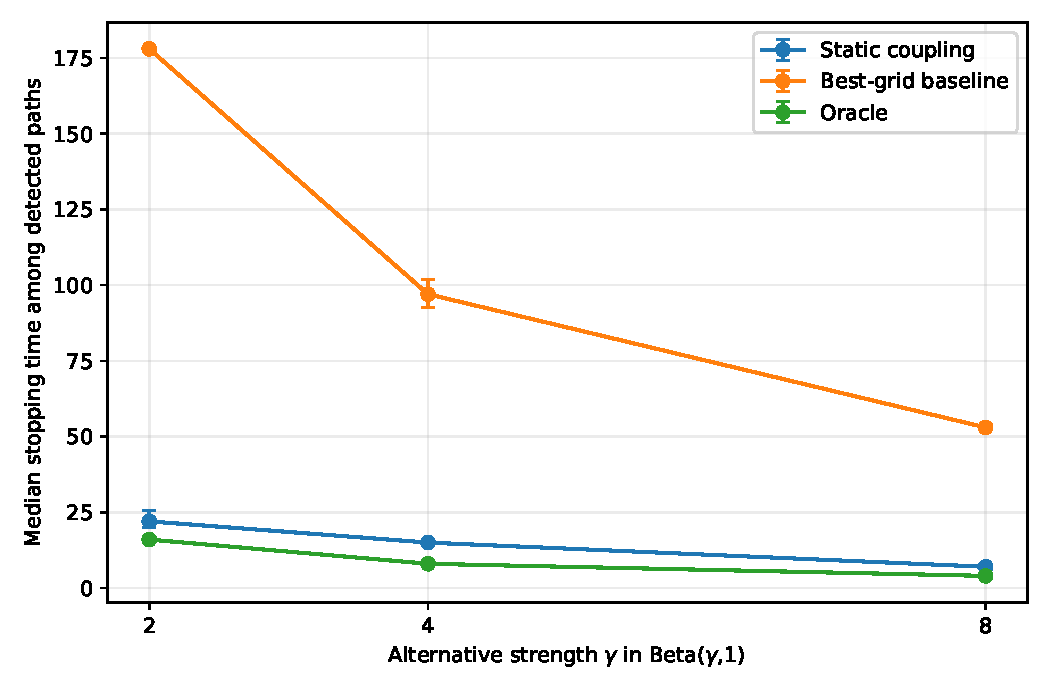
\includegraphics[width=0.82\linewidth]{../results/publication_v1/figures/delay_T200_K32.pdf}
\caption{Median stopping time among detected paths for \(K=32\), with bootstrap 95\% intervals. Delay is conditional on crossing and should be interpreted jointly with crossing probability.}
\label{fig:delay-k32}
\end{figure}

\subsection{Evidence diagnostics and tuning}

At \(K=32,\gamma=4,T=200\), median terminal log evidence is \(9.4131\) for static coupling and \(13.3054\) for the oracle. The selected best-grid comparator is the fixed band mixture at \(\delta=0.045\), with crossing probability \(0.1152\), median terminal log evidence \(-1.4528\), and threshold approximately 191.

At \(K=32,\gamma=8,T=200\), corresponding static and oracle median terminal log evidences are \(28.3517\) and \(34.3784\). The selected best-grid band mixture at \(\delta=0.045\) reaches crossing probability \(0.8362\) with median terminal log evidence \(20.1043\). These values are diagnostic only because the confidence-band thresholds differ from 20.

The selected baseline differs across conditions because the reported comparator is deliberately the strongest ex-post member of the frozen grid. This makes it a descriptive adversarial benchmark rather than one precommitted level-\(\alpha\) test.

The publication-scale run preserves the qualitative conclusions of the earlier 200-rep development audit without changing the method. Representative static crossing estimates move from \(0.880\) to \(0.8758\) for \(K=24,\gamma=4\), from \(0.935\) to \(0.9144\) for \(K=32,\gamma=4\), and from \(0.195\) to \(0.2036\) for \(K=32,\gamma=2\). Likewise, the \(K=32,\gamma=8\) best-grid baseline changes only from approximately \(0.840\) to \(0.8362\).

\subsection{Interpretation}

A confidence-band method asks which null CDFs remain compatible with the contaminated reference. Static coupling asks which \emph{single persistent set of contaminated identities} could explain the entire repeated rank history. The experiments suggest that preserving this persistent combinatorial constraint can retain substantially more usable finite-reference evidence, especially in the moderate-shift regime.

\section{Discussion}

\subsection{Persistent latent structure}

The proposed construction exploits persistent latent structure. A confidence-band robustification asks which null distributions remain compatible with the contaminated reference data and thereby forgets which individual reference observations might be contaminated. Static coupling retains that uncertainty as one fixed latent candidate set
\[
  C\subseteq\{1,\ldots,K\}
\]
that is reused at every future time.

The distinction is therefore not simply \emph{rank method versus CDF method}. It is a distinction between \emph{persistent latent identity uncertainty} and \emph{generic distributional uncertainty}.
The lower envelope can still be conservative, but it preserves the constraint that one contamination pattern must explain the entire online rank history.

\subsection{Relation to the oracle}

At the primary frozen setting
\[
  K=32,\qquad m=2,\qquad \gamma=4,\qquad T=200,
\]
the oracle crossing probability is \(0.9810\). Static coupling reaches \(0.9144\) in the original outside-support geometry and between \(0.8894\) and \(0.9468\) across the three pre-specified non-control geometries. The corresponding oracle-static point gaps are \(0.0666\), \(0.0916\), \(0.0388\), and \(0.0342\).

The invariant oracle result across V1b geometries is a useful structural check: the clean reference and future stream are held fixed, and a correct oracle removes the contaminated sorted positions before applying the same clean-rank construction. Geometry affects the robust and confidence-band procedures, but not the underlying canonical clean rank sequence.

We do not derive an analytical efficiency bound for the oracle-static gap. Characterizing its dependence on \(K\), \(m\), horizon, and alternative strength remains open.

\subsection{What V1b changes}

The geometry stress test rules out a simple explanation of the original power gap: that both contaminants at value \(2\) created an unusually favorable setting for static coupling. The fixed confidence-band comparator improves substantially when contaminants are moved into the support or split across tails, rising from \(0.1152\) to as high as \(0.3948\) at the primary point. The static method nevertheless remains between \(0.8894\) and \(0.9468\).

This does not establish uniform dominance over all geometries. It does show that the main empirical finding survives a pre-specified set of materially different static/exogenous contamination arrangements without changing the detector.

\subsection{Why the band comparison is conservative}

The confidence-band baselines represent the contaminated reference through a simultaneous CDF uncertainty set. This remains valid without identifying contaminated positions, but the resulting uncertainty set can be substantially larger than the set compatible with one persistent contamination pattern. The final development audit intentionally favors the band family by sweeping a frozen parameter grid and reporting the best configuration ex post for each condition.

Because the ex-post envelope is not one precommitted test, it is used only as a descriptive adversarial benchmark. V1b fixes \texttt{band\_mix}, \(\delta=0.045\), before its geometry outcomes and reports paired Monte Carlo uncertainty against that comparator. Because the comparator was informed by the earlier Publication V1 analysis and the V1b control reuses those paths, these intervals are not presented as selection-adjusted confirmatory inference.

\subsection{Marginal versus conditional guarantees}

Theorem~1 inherits the marginal fixed-reference interpretation of predictive-rank martingales \cite{KuangXia2026}. It averages over the random clean reference sample. CCTM instead targets a calibration-conditional guarantee with high probability over a clean reference draw \cite{ShaerEtAl2026}. These are different inferential targets. We do not claim that one uniformly dominates the other.

\subsection{Connection to CFAR and receiver data}

The radar motivation is direct but limited. Classical CFAR uses neighboring reference cells to set a threshold for a cell under test, with order-statistic and censored variants addressing nonhomogeneous windows and multiple interferers \cite{Rohling1983}. Our setting instead reuses one finite reference bank repeatedly, permits persistent contaminated cells, and requires optional-stopping-safe sequential evidence.

The semi-synthetic RTL-SDR experiments provide an engineering bridge rather than a theorem check. Real receiver/background IQ preserves quantization and environmental structure, while controlled post-ADC injection preserves known ground truth. V2 exposes a non-saturated transition: at \(-18\) dB static crosses on 14/30 captures versus 0/30 for the fixed band comparator, and at \(-15\) dB the corresponding counts are 22/30 versus 12/30. These observations are qualitatively consistent with the simulation advantage, but serial dependence prevents interpretation as hardware type-I validation.

\subsection{Structural versus distributional robustness}

The model illustrates a broader distinction. Distributional robustness enlarges the set of possible laws. Structural robustness can exploit restrictions on how nuisance variables persist. Here the nuisance parameter is not a new arbitrary corruption at every time; it is the fixed set \(C^\star\) shared by all future comparisons. The theorem itself is simple once that structure is stated, but recognizing and preserving this constraint is what makes the construction useful.

\subsection{Computational considerations}

Exact enumeration requires
\[
  \binom{K}{m}
\]
candidate processes. This is practical for the frozen experiments with \(m=2\), but does not scale well when both \(K\) and \(m\) increase. The contiguous-partition dynamic program solves the fixed-categorical case in \(O(Km^2)\) time and \(O(Km)\) memory. The full frozen convex portfolio lacks the same additive structure, so no polynomial-time exact algorithm is claimed for it.

\subsection{Finite-reference information ceiling}

For fixed \(n\),
\[
  P\sim\mathrm{Dirichlet}(1,\ldots,1),
  \qquad
  R_t\mid P\overset{\mathrm{iid}}{\sim}\mathrm{Categorical}(P).
\]
As the online horizon grows, the stream increasingly reveals the realized spacing vector \(P\), but does not eliminate randomness from the finite reference itself. Some persistent rank patterns under alternatives can therefore remain compatible with rare null spacing realizations. This finite-reference ceiling is consistent with the limitation identified for clean PRMs by Kuang and Xia \cite{KuangXia2026} and motivates our focus on finite-reference power rather than universal fixed-\(n\) consistency.

\section{Limitations and Future Work}

\paragraph{Exact contamination count.}
The theory and frozen experiments assume that the exact number \(m\) of contaminated references is known. A lower envelope over candidate sizes \(0\le r\le M\) is a natural extension when only an upper bound is available, but each size changes the clean-reference count and predictive null law.

\paragraph{Static/exogenous contamination.}
The theorem requires that deleting the true contaminated cells leaves an iid clean reference sample. It does not cover value-adaptive replacement chosen after inspecting clean realized values. Such selection can bias the surviving clean subset.

\paragraph{Scalar continuous observations.}
The theorem assumes scalar observations from a continuous null. Quantized, discrete, vector, complex-valued, and tied data require additional construction, such as randomized ranks or application-specific scalar scores.

\paragraph{Independence and stationarity.}
Clean references and future null observations are iid from the same unknown \(F\). Temporal dependence, drift, and reference/test mismatch are outside the current theorem and are particularly relevant in RF sensing.

\paragraph{Frozen contaminant geometry.}
The primary simulations place two contaminants at value 2, outside the support of the clean null and alternatives. Publication validation should also include in-support, mixed-tail, and random static contaminants without changing the frozen detector.

\paragraph{Monte Carlo precision.}
The final development audit uses 200 replications per condition. This is adequate for the large exploratory gate but modest for publication-quality uncertainty estimates. A post-freeze validation pass should use substantially more replications and report uncertainty intervals while keeping every method and tuning parameter unchanged.

\paragraph{Baseline scope.}
The contaminated-reference confidence-band comparators are our adaptations of clean-reference DKW/CCTM ideas. They are neither canonical nor optimal contaminated-CCTM procedures. The empirical claim is therefore limited to the tested valid adaptations.

\paragraph{No optimality claim.}
The lower envelope is valid, but no minimax or uniformly most powerful property is proved. Better betting families or candidate aggregation strategies may exist.

\paragraph{Full-mixture optimization.}
The polynomial dynamic program applies only to a fixed categorical bettor. The complete frozen portfolio is evaluated by enumeration. Scalable exact or certified approximate optimization is future work; any approximation used for testing must preserve a conservative lower bound compatible with Theorem~1.

\paragraph{RF validation.}
The mathematical theorem does not require hardware data. For an engineering audience, however, a semi-synthetic RTL-SDR experiment can provide external validation using real receiver IQ plus controlled offline contamination and signal injection. Such an experiment would test whether the qualitative finite-reference behavior survives quantization, front-end imperfections, and environmental RF. It would not constitute a proof of the theorem or a claim of universal field performance.

\section{Conclusion}

We studied anytime-valid sequential detection when a finite fixed reference bank is already contaminated before monitoring begins. The defining feature is persistence: the same unknown contamination identities are reused at every future comparison.

Building on the clean fixed-reference predictive-rank martingale of Kuang and Xia \cite{KuangXia2026}, each candidate contamination set induces a reconstructed rank sequence. For the true candidate,
\[
  R_t^{(C^\star)}=R_t^{\mathrm{clean}},
\]
so its candidate wealth is a valid clean PRM. The lower envelope
\[
  \underline E_t=\min_C E_t^{(C)}
\]
satisfies the pathwise inequality
\[
  \underline E_t\le E_t^{(C^\star)},
\]
which yields
\[
  \Pr_{H_0}\!\left(
    \sup_t\underline E_t\ge\frac1\alpha
  \right)\le\alpha.
\]
The lower envelope itself need not be an e-process; its guarantee follows from domination by the true-candidate process.

Static contamination also induces a contiguous-partition representation of observed-rank bins. For a fixed categorical bettor, this structure leads to an exact \(O(Km^2)\)-time, \(O(Km)\)-memory dynamic program. A corollary extends validity to an unknown contamination count bounded by \(M\), and the finite-reference asymptotic analysis explains why the frozen finite portfolio need not accumulate unbounded evidence for every persistent alternative when the reference size is fixed.

In the frozen simulation study, persistent-identity coupling retains substantially more finite-reference power than the tested confidence-band robustifications. At
\[
  K=32,\qquad m=2,\qquad T=200,\qquad X_t\sim\mathrm{Beta}(4,1),
\]
the observed crossing probabilities in 5,000 post-freeze replications are \(0.9144\) for static coupling, \(0.1152\) for the strongest ex-post frozen-grid confidence-band benchmark, and \(0.9810\) for the oracle. The paired static-minus-baseline gap is \(0.7992\) with 95\% bootstrap interval \([0.7880,0.8104]\), while median detected stopping times are 15, 97, and 8.

The conclusion is deliberately narrow: when contamination is static, preserving persistent identity structure can provide finite-reference information that is lost when uncertainty is represented only through a generic CDF band. The result is not a claim of universal robustness or superiority; it applies to the stated static/exogenous model and inherits the marginal fixed-reference interpretation of predictive-rank martingales. Semi-synthetic RTL-SDR validation is the next step toward establishing whether the same qualitative behavior survives a physical receiver chain.


\bibliographystyle{plain}
\bibliography{references}

\end{document}
